\documentclass[thesis.tex]{subfiles}
\begin{document}
\chapter{Introduction}

%\todo{%
%  This chapter should introduce:
%  \begin{itemize}
%  \item Introduce the thesis.
%  \item State the main contributions.
%  \end{itemize}
%
%  We should also ask \emph{what is the thesis of the thesis} which is a fiddly
%  way of asking what are we trying to prove with this document?
%}

\begin{figure}
  \centering
  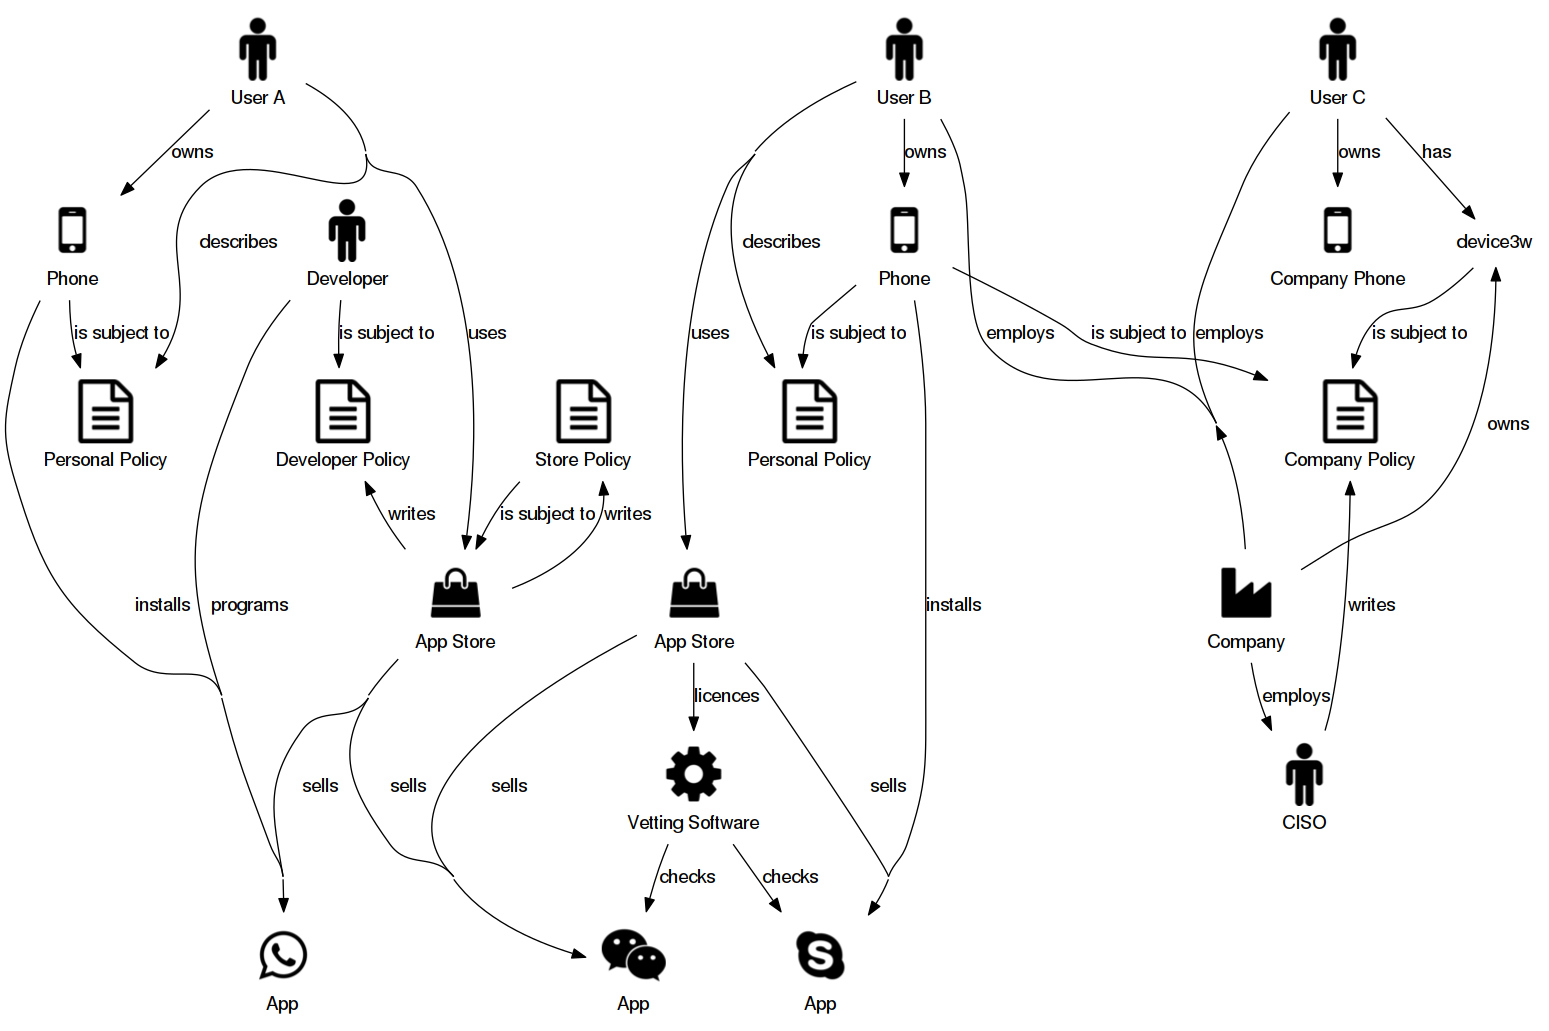
\includegraphics[width=\linewidth]{figures/mobile-ecosystem.png}
  \caption{Interactions surrounding the use of mobile devices.}
  \label{fig:mobile-ecosystem}
\end{figure}

Mobile devices are ubiquitous, yet the relationships between their users, and
the environment they run in is often vague. Users have preferences for the apps
they use. Stores have terms for the apps they sell, and for the users who buy
them. Companies have policies as to what apps and devices employees can use in
the office. The precise trust relationships, however, are often hidden in
informal, or natural language, descriptions of the policies.

As the devices have become more powerful, there has been an increasing wish to
control the devices. Companies expect devices to follow their corporate policies
within their networks and trust users to abide by their policies as well as use
tools to enforce some aspects of them. Some users may have reservations about
what data an app can get access to and may wish to restrict the app's access.
Users may rely on stores to vet the apps they sell, but will likely not know (or
necessarily care) precisely how the store checked the app.

These devices exist within the \emph{mobile ecosystem}: which we
define as \textbf{the interactions surrounding the use of smart phones
and tablet computers in a given
setting}. Figure~\ref{fig:mobile-ecosystem} shows some relationships
between devices, their users and their preferences, the stores,
companies and all these principal's policies. Users have phones or
other mobile devices. The users may own personal or have company
provided devices. They may have their own preferred ways of using the
device, or they have to follow policies written by their
employer. Users download apps, written by developers, from app stores;
each store has their own policies and some stores may delegate some
aspects of their quality control to external vetting software.

Prior work focused on how systems and tools can check and enforce more
sophisticated policies and ever finer controls. This thesis asks a different
question: \textbf{how can we capture the informal policies and trust
relationships surrounding the mobile ecosystem and use formal languages to model
and examine them?} We ask how can we tie the top-level goals in the natural
language policies and preferences to the tools used to implement them? How can
we compare different policies and highlight similarities and differences between
them precisely?

\section{The Policies of the Mobile Ecosystem}

As mobile devices are increasingly capable and hold ever-increasing amounts of
information, users and businesses need to manage how the devices behave.
Employees now bring their mobile devices to work and use them to access company
email and documents. In response to this companies might \emph{mandate} that
employees follow mobile device policies that describe how the employees should
use their devices within the company. These policies vary in terms of formality
inside and outside of a company. 
They may also use \ac{MDM} software, tools which allow companies to configure
mobile devices remotely, to enforce the policies. Regulation, such as
\ac{HIPAA}, may also affect some companies.

A user may never write their personal privacy preferences in a formal language
but they may make decisions guided by them. An example might be a user choosing
which apps to install and which to avoid, based on their own \emph{discretion}.
They may make decisions based on what their friends have told them, or what a
review said about the app.

In this section we will start to introduce by example AppPAL: an authorisation
language for the policies of the mobile ecosystem, and is based on
SecPAL~\cite{becker_secpal:_2006}. We will describe AppPAL in greater detail in
\autoref{chap:apppal} and throughout the thesis, but it is, in essence, an
instantiation of the SecPAL system to the mobile domain, along with some minor
changes to syntax. We have implemented AppPAL to explore its use and to capture
the policies of the mobile ecosystem. Whenever we show an AppPAL snippet in
\framebox{\texttt{teletype font}} it can be parsed and used as part of a
policy\footnote{Sometimes with minimal edits as some constraints used are not
implemented.} with our implementation.

An AppPAL policy consists of many assertions.  Each assertion is a statement by
a principal either of a fact, or a rule for inferring a fact.  For example, the statement:
\begin{lstlisting}
'alice' says 'angry-birds' isGood.
\end{lstlisting}
Should be read as an assertion by Alice (a principal), that Angry Birds (a
constant) is good (a predicate).  An example of a rule might be:
\begin{lstlisting}
'alice' says App:A isGood 
  if A isFree.
\end{lstlisting}
This example should be read as an assertion by Alice that any App (a type),
referred to as A (a variable) is good if A is also free (a conditional).   

As well as assertions about whether variable or constant subjects meet certain
predicates, AppPAL can be used to describe delegations, such as:
\begin{lstlisting}
'alice' says 'bob' can-say App:A isGood.
\end{lstlisting}

\pagebreak
Which should be read as an assertion by Alice that if Bob says an App, A, is
good then she will also agree that it is good.  AppPAL can also describe roles,
the assertions:
\begin{lstlisting}
'alice' says 'polygon.com' can-say X isGood.
'alice' says 'justin' can-act-as 'polygon.com'.
\end{lstlisting}
Are read as first an assertion by Alice that she trusts \url{polygon.com} (a
famous video-game news website) to say whether something, referred to as X, is
good; and secondly as an assertion that Alice allows Justin (one of
\url{polygon.com}'s editors) to act as the website.  

A full description of AppPAL will be given later in the thesis.  
AppPAL inherits its evaluation rules and semantics from SecPAL which is described in
\autoref{sec:secpal}.  AppPAL's syntax, however, differs slightly
from SecPAL and includes some conventions for writing policies---these changes
are described in \autoref{sec:instantiating}.

A key aspect of the mobile ecosystem is \emph{delegation}. The user of a mobile
device (typically) first logs on to a Google or Apple account before using the
device, which fetches all their data from a server on the internet. Rather than
keep account information locally an app may prompt the user to log in,
delegating to a third-party (such as Google or Facebook) to manage the account
ID. Capturing these trust relationships as policies can help clarify the precise
terms for authentication and who each principal trusts to make what decisions.
For example, an app might trust Google to manage accounts. Google will only
authorise a user if the user has authorised the app, and will only allow the app
access to the data the user has explicitly authorised:

%\noindent\begin{minipage}{\linewidth}%\vspace{\baselineskip}
\begin{lstlisting}
'app' says 'google' can-say 
  'app' canLink(User:U, Account:A).

'google' says App:A canLink(User:U, Account:Acc)
  if U hasAuthorized(A), U hasAccount(Acc).

'google' says User:U can-say U hasAuthorized(App:A)
  if U isAuthenticatedWith(Token), Token isValid.

'google' says User:U can-say App:A canAccess(Data:D)
  if D isOwnedBy(U).
\end{lstlisting}
%\end{minipage}

Users may install apps manually themselves, but they might also buy and download
apps from one or more app stores. They trust these app stores to sell them
\emph{good and safe} apps, and delegate the checking of them to the store.
Whereas, in the earlier days of PCs, a user might once have done the check
themselves (or at least delegated to an \ac{AV} package on their computer) now
the responsibility is with the stores. Now most apps come signed either by the
developer who created it (in the case of Google's Play Store), the store that
sold it (in the case of Amazon's app store) or both (Apple's App Store). These
signatures ensure integrity and some measure of authenticity, standing for an
assertion that the signer makes that the app is safe to run. For example we may
take Apple's signature as an assertion that Apple's vetting process has approved
the app is safe to use by its customers. A store may delegate to a third-party
app vetting service to assess what apps are safe (Yandex and Aptoide stores), or
use their own in-house teams.

Users sometimes recommend apps to each other. We can capture, for example, that
Alice may trust Bob to tell her which apps are good.
%
\begin{lstlisting}
'alice' says 'bob' can-say App:A isGood.
\end{lstlisting}
%
Some may consider what apps they want to use on their phone and come up with
informally applied personal policies that describe how they want to use them.
They may never write these policies down, but they might take the form of
preferences that influence the apps they choose, by capturing these we can start
to examine and compare policies as well as potentially enforcing them. Bob might recommend any app by Nintendo:
%
\begin{lstlisting}
'bob' says App:A isGood
  if A isGame,
     A hasDeveloper('nintendo').
\end{lstlisting}
%
Bob might trust reviews and review sites to give him an idea of an app's quality. 
%
\begin{lstlisting}
'bob' says App:A isGood
  if A hasReviewScore(N)
  where N > 60.
 
'bob' says 'metacritic' can-say
  App:A hasReviewScore(Percent:N).
\end{lstlisting}

\pagebreak
Bob might also recommend an app based on its app store categorisation and its permissions.
%
\begin{lstlisting}
'bob' says App:A isGood
  if A hasCategory('flashlight'),
     A hasPermissions(P)
  where ! contains(P, 'INTERNET').
\end{lstlisting}

Users allow their employers to say how they should their devices, who
may in turn delegate to IT departments, to write rules, which may
delegate back to the users to state what rules they're willing to
follow.

A company looking to control their employee's mobile devices at work
might write a \ac{BYOD} policy that their employees agree to
follow. They might also use \ac{MDM} software to control some aspects
of their devices. The company might write these with varying degrees
of formality but often they use natural language. This adds vagueness
and can lead to confusion about how the company upholds the policy. By
describing the policy in a formal language we can express the policy
rigorously. We can start to make comparisons between users, and with
rules for checking the policy start to help the user to make decisions
more accurately, or measure the extent a user follows their stated
policy. Using formal languages we can model the policies precisely,
helping clarify their meanings and make precise comparisons between
different policies. We could tie the rules in the \ac{BYOD} policies
to the \ac{MDM} tools used to check them.

In the US all software for use with medical data must conform to a policy
called \ac{HIPAA}, and this includes apps on mobile devices.  The \ac{HIPAA}
act covers many rules specific to medical software including requirements for
keeping medical records confidential.  If a company needs its employees to use
such apps they could use static analysis tools to check for some aspects of the
\ac{HIPAA} policy.  A company might use Mallodroid~\cite{fahl_why_2012} to
detect when apps send data unencrypted.  
%
\begin{lstlisting} 
'company' says Employee:E canUse(App:A) 
  if A isHIPAAConformant 
  where mallodroidCheckSafe(A) = True. 
\end{lstlisting}


It is important not to confuse the tools and techniques we might use to uphold
parts of a policy with the end goal of ensuring compliance.
%
A taint-tracking tool, like TaintDroid~\cite{enck_taintdroid_2010} (for
example), can tell when sensitive data is being leaked out of a network socket.
If the end security goal is to prevent employees leaking data, this only covers
part of the policy---what about a malicious employee stealing files by printing
them and walking out of the office with them?  How do we run the tool and when?
Using a tool to check for compliance does not necessarily mean that a policy is
fully implemented.
%
A formal language that lets us sever the policy from its implementation can
help us understand the policy precisely, and show precisely how we check
the policy.  It lets us see which tools are checking what rules, and identify
gaps where the policy is not being checked sufficiently.

These trust relationships and delegations permeate the entire mobile
ecosystem.  They represent an important aspect of the ecosystem that a
policy language should catch to describe the
relationships and policies within it.

In this thesis we will come back to these ideas of user's personal
privacy policies and \ac{BYOD} policies as they show two different aspects
of how policies are used within the mobile ecosystem.
%
User's privacy preferences are very informal and may not be something
a user would ever consider writing down.  Rather, a user's privacy
preferences guide which apps they might use. A user might even be
willing to use an app that does not match their preferences in some
cases, such as using the Facebook app (which can access lots of data
on a user's device) whilst being generally unhappy sharing their data
with their software.
%
In contrast a \ac{BYOD} policy can exist as a formal agreement (though
often \emph{informally} specified) between the company and its
employees.  An employee might reasonably expect to face consequences
if their employer discovers they broke the \ac{BYOD} rules.

Superficially these policies also resemble classic \ac{DAC} and \ac{MAC}
policies. A company \emph{mandates} the \ac{BYOD} policy, the user uses
their \emph{discretion} when picking the apps they use on their phone.
An interesting aspect of the mobile ecosystem is that the policies are
more complicated than simple \ac{MAC} and \ac{DAC} distinctions and use aspects
of both.  In \autoref{chap:byod} we will look at how companies use
employee's discretion to judge if aspects of the company's \ac{BYOD}
agreements (such as ethical policies) have been followed.  

In contrast, users use their discretion to follow their privacy
preferences when picking and using apps.  The user must decide whether
an app has the need to access certain device functionality or be
installed on their phone at all.  A user using a \emph{fine-grained
permissions system} (such as one described in
\autoref{sec:fine-grained-permissions}) or creating a curated app
store (we give a method to do so using a policy in
\autoref{sec:an-apppal-enhanced-store}). Now the user will end up
writing a \ac{MAC}-style policy describing how their phone should
behave and what apps the store should sell.

\ac{BYOD} policies and privacy preferences are only a subset of the
policies we might see in the mobile ecosystem.  We will survey some
other policies in the course of the thesis including app store terms
and conditions, and the app signing models built into the mobile OSs,
but we chose to focus on \ac{BYOD} and privacy preferences as they covered
a range of policy styles, high and low-level policy topics and could
showcase some of what makes the mobile ecosystem fascinating.

\section{Capturing Mobile Security Policies Precisely}
\label{sec:methods}

The topic of this thesis is how can we capture the informal policies
and trust relationships surrounding the mobile ecosystem and use
formal languages to model and examine them?  Existing research on
mobile security policies has focused on enforcing app permissions
policies---the \emph{fine-grained} permissions systems.  These
permission systems allow for new and powerful ways of expressing how
users want their devices to behave, but they do not deal with the fact
that users say not typically express their policies in terms of
permission sets or formal policies but instead might use natural
language.

Existing work has given us the mechanisms for enforcing
arbitrary mobile security policies, but not the means to link them
back to the human natural language informal policies people use in
practice.  What existing research lacks is the mechanisms to capture
and reason about the informal policies precisely, and then link them to
the tools and mechanisms that can enforce them.

With the goal of showing how to capture the informal mobile security
policies precisely in mind, this thesis attempts to answer the
following research questions:

% Research questions
\begin{itemize}
\item \emph{How can we capture precisely an informally specified
    mobile security policy using a formal language?}
  
  This is the central question of the thesis.  We propose using an
  authorisation logic as a formalisation to capture mobile device
  policies as these logics have been previously used to capture
  policies.  Based our requirements for the language and a survey of
  existing policy languages we suggest using a SecPAL-based language
  (AppPAL).  The rest of the thesis contains various case-studies where
  we show that our proposed language can capture the policies and give
  us greater insight into their rules and provide potential enforcement
  mechanisms.
    
\item \emph{Do we see personal app privacy preferences reflected in
    users' choice of apps?}
  
  To answer this question we have access to data about users policies
  and app installations---therefore we use quantitative research methods
  as AppPAL gives us a mechanism to query policies against data.

  Existing work has identified 4 generalised app privacy preferences
  people state they follow~\cite{lin_modeling_2014}.  Existing work has
  also created a data-set of what apps users
  installed~\cite{oliner_carat:_2013}.  To answer this question we
  encode the stated privacy preferences as AppPAL policies, then use
  AppPAL to find the apps that would be accepted by the policy.  The
  extent a user is following the policy is found by measuring
  quantitatively the percentage of apps that the user has installed that
  met the policy as a percentage of the apps they installed overall.

\item \emph{What are the common decisions in \ac{BYOD} policies, and
    are these the decisions that \ac{MDM} tools help to enforce?}

  This question lets us use AppPAL for a case-study into \ac{BYOD}
  policies.  We do not have access to any data about \ac{BYOD} usage,
  but we can examine the policies.  The research methods used to answer
  the question are encoding into AppPAL (for the policies) and survey
  for the functionality of the \ac{MDM} tools.  This allows us to
  further explore the policies on the basis of our encoding, without
  having to deal with the ambiguity of natural language policies.
  
  We take various \ac{BYOD} policies and express them in AppPAL.  This
  can be somewhat subjective, so care must be taken to capture the style
  and intent of the original policy and to use a consistent set of
  predicates between policies.  With the policies encoded in AppPAL we
  can look for common decisions, idioms and trust structures and make
  comparisons precisely on the basis of the formal version of the
  policy.  We survey the features of various \ac{MDM} tools by examining
  their websites and documentation.  Finally we contrast what \ac{MDM}
  tools can do with the decisions that \ac{BYOD} policies want to make.
\end{itemize}


% Existing limitations

\subsection{Thesis Outline and Publications}

The rest of this thesis is organised into the following chapters.  Some work
described has been presented at various conferences, workshops and PhD
symposiums through the course of the PhD.  We describe the publications, and
show where they fit into the various chapters.

For each of our publications the work described was done by the first
author: Joseph Hallett (\emph{me}, the thesis author).  The second
author, Professor Aspinall (my PhD supervisor), provided invaluable
suggestions and advice as to where to go with the research as well as
extensive editing.

\begin{itemize}
\item \textbf{Chapter 2: Background.}  This chapter describes
  Becker~\etal's work on SecPAL, and gives an overview of work on other
  policy languages including XACML and DKAL as well as the fine-grained
  permission systems used to enforce policies on Android devices.

\item \textbf{Chapter 3: Instantiating and Evaluating SecPAL.}  The
  next chapter introduces AppPAL as a language instantiating SecPAL to
  describe the policies of the mobile ecosystem. We introduce the
  language through examples before showing how we implemented it. We
  also describe some modifications to the language from SecPAL to make
  writing policies easier. We conclude by describing our tools for
  analysing AppPAL policies for satisfiability and redundancy errors.
  
  Some early examples were taken from our paper:
  \begin{itemize}
  \item\emph{Towards an authorisation framework for app security
      checking~\cite{hallett_towards_2014}.} This is a PhD symposium paper that describes how
    we might use SecPAL to model policies in the mobile ecosystem.
  \end{itemize}

\item \textbf{Chapter 4: App Stores and App Preferences.} 
  Having described AppPAL, this chapter starts to describe the differences between different
  app stores and survey their different terms and conditions. We use AppPAL to
  capture descriptions of user's app privacy preferences; and measure the extent
  users follow these preferences when selecting apps by comparing with records of
  user's app installation history. Finally, we describe a tool for generating
  \emph{curated} app stores on the basis of a policy.
  
  The implementation described, and work on capturing user's privacy preferences is included in our papers:
  \begin{itemize}
  \item\emph{AppPAL for Android~\cite{hallett_apppal_2016}.} This
    conference paper describes AppPAL as an instantiation of SecPAL.  We
    present AppPAL evaluation algorithm, and show how to capture user
    privacy preferences as AppPAL policies. We use the AppPAL versions of
    the privacy policies to find examples of users following the policies
    in a user app-installation data set.
  \item\emph{Poster: Using Authorisation Logic to Capture User
      Policies in Mobile Ecosystems~\cite{hallett_poster:_2015}.}  This
    poster presents early work measuring the extent users seem to follow
    an AppPAL translation of user privacy preferences.
  \end{itemize}

\item \textbf{Chapter 5: Applying AppPAL to \ac{BYOD} Policies.}
  We move from describing \emph{user-centric} policies, to ones companies might
  want to enforce. We look at how we can capture \ac{BYOD} policies using AppPAL by
  looking at 5 \ac{BYOD} policies (which are included in Appendix A). In capturing the
  policies, we identify two idioms that existing MDM tooling does not capture. We
  also describe how AppPAL could be used to enforce a \ac{BYOD} policy by integrating
  with existing tooling.
  
  This chapter encompasses and extends our work presented in:
  \begin{itemize}
  \item\emph{Capturing Policies for
      \ac{BYOD}~\cite{hallett_capturing_2017}} This conference paper shows
    how AppPAL can be used to capture the rules and trust relationships in
    \ac{BYOD} policies.
  \item\emph{Common Concerns in \ac{BYOD}
      Policies~\cite{hallett_common_2017}.} This conference paper looks at
    \ac{BYOD} policies and our efforts to find common areas of concern
    within them.
  \item\emph{Specifying \ac{BYOD} Policies with Authorisation
      Logic~\cite{hallett_specifying_2016}.} This PhD symposium paper
    describes early work capturing \ac{BYOD} policies with AppPAL.  The
    paper describes how we could use AppPAL to look for common problems,
    such as completeness.
  \end{itemize}

\item \textbf{Chapter 6: Future Work.}
  This chapter describes possible future work, including a probabilistic variant of AppPAL.
 
\end{itemize}

\subsection{Research Contributions}

This thesis makes the following contributions:

\begin{itemize}
  \item I show how SecPAL can be instantiated with predicates and conventions
    to create a language called AppPAL to describe the policies of the mobile
    ecosystem.
  \item I provide an open source implementation of SecPAL and AppPAL. This also
    contains tooling for examining policies for common problems such as
    consistency and redundancy.  The previous implementation (by the authors of
    the SecPAL paper~\cite{becker_secpal:_2006}) is closed source, and runs
    only on Windows.  Our implementation is written in Java and will run in the
    JVM and on Android devices.
  \item I describe a framework for measuring the extent users follow policies
    with respect to their app choices.  Using this framework and a collection
    of app privacy policies found by surveying users~\cite{lin_modeling_2014},
    I show that users do not seem to follow them in practice.
  \item I provide a table summarising the differences in terms and conditions
    between 5 different app stores.
  \item I provide a formal version of 5 different \ac{BYOD} policies, written in
    AppPAL.  Using the formal versions of the policies to compare the contents
    of the policies I identify two idiomatic forms of \ac{BYOD} policy rules that
    have not been examined before or supported by existing tooling.
\end{itemize}

It is difficult to judge the extent the investigations in this thesis have been
a success.  We do not, for the most part, provide any proofs that could be
checked to show our AppPAL policies are correct, more precise and more powerful
than the natural language ones we claim to capture.  In fact, the act of writing
down the policies in AppPAL requires a degree of subjectivity to capture the style
and intent of the original policy. It would be reasonable to look at some of
our policies and say that a different version might be more accurate or more
descriptive.

As well as describing the policies, this thesis also describes how we can
compare and analyse the policies. The AppPAL language give us rules and a
grammar for capturing the policies, decisions and trust relationships of the
mobile ecosystem.  You might not like our versions of the policies. If you can
use AppPAL to describe what a better version of the policy might be, however,
then our version of the policy provides a baseline to compare against and our
methods let us see whether we would find new or different results with the
improved policies.

% TODO: I hate this fix it.  Too cute.
One approach to judging this work is to consider what the act of capturing the policies in a formal language lets us do.
We believe that expressing mobile security policies precisely lets us see the trust relationships more clearly.
It allows us to make comparisons on the basis of a formalisation.
It helps us understand and argue about the policies.
If by capturing the mobile security policies, what we learn is interesting and leads to worthwhile discussion, then our investigations are a success.
Alternately if what we have discovered is trivial, wrong, and our language
fails to capture the policies in any way, then this work must be judged a failure.

I believe the former is the case.  This work is interesting. We do manage to
capture the trust relationships of the mobile ecosystem successfully.

\end{document}


%%% Local Variables:
%%% mode: latex
%%% TeX-master: "../thesis"
%%% End:
